\subsection{Arquitectura  del servidor}

El servidor se ha implementado con Spring Boot \cite{spring}, un framework que permite la creación de aplicaciones en Java de una forma más sencilla. En cuanto a la base de datos a la que se conecta, se trata de una base de datos NoSQL, donde los datos están orientados hacia el almacenamiento de documentos. En este caso se ha utilizado MongoDB.

\begin{figure}[H]
\centerline{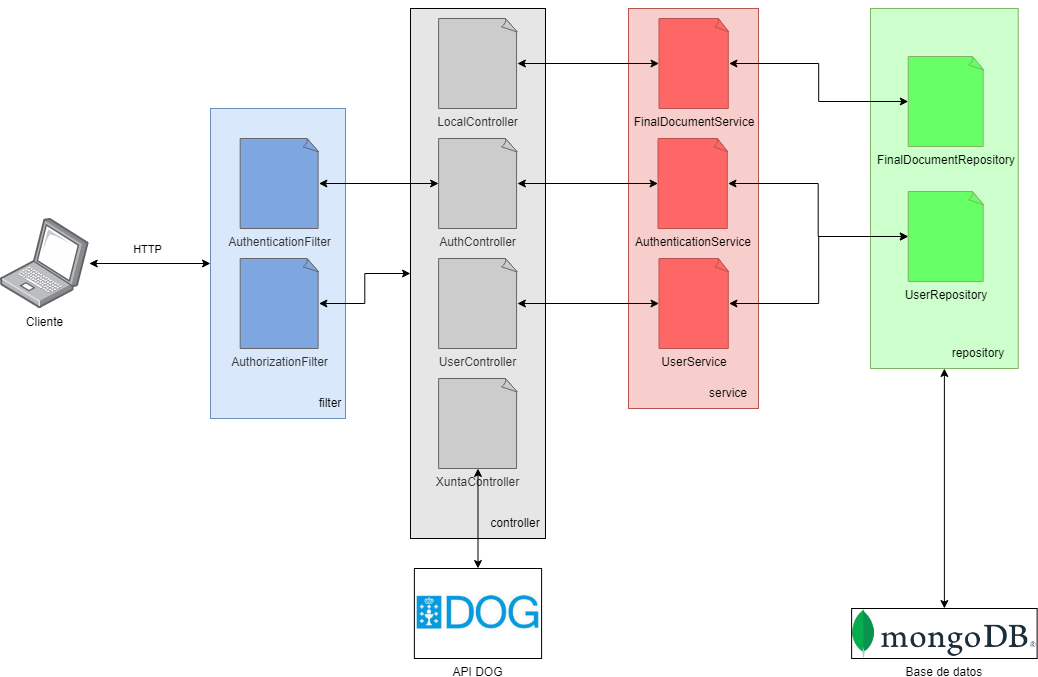
\includegraphics[width=15cm]{figuras/diseño/FicherosServidor.png}}
\caption{Arquitectura del servidor.}
\label{enlaceArquitecturaServidor}
\end{figure}

El servidor está dividido en un conjunto de directorios, cada uno con una función diferente. 
\\

En el directorio Config, se localizan archivos de configuración del propio servidor, tales como aspectos de seguridad, documentación, privacidad, etc. 
\\

Otro directorio es el de Filter, donde se tratan distintos aspectos de seguridad con respecto a los usuarios que utilizan la aplicación, como puede ser el inicio de sesión, gestión de contraseñas o comprobación de roles.
\\

En la carpeta Model encontramos los distintos objetos que conforman la base de la aplicación. Podemos destacar entre ellos el objeto FinalDocument, que está formado por todos los atributos de la ley, y User, que es el objeto utilizado para gestionar los usuarios.
\\

En la carpeta Controller, encontramos todos los archivos encargados de redirigir las llamadas a los servicios necesarios en la carpeta Service. Estos se encargan de localizar cualquier llamada al servidor (GET, POST, ...), y entregarla a los servicios. Además, existe un controlador (XuntaController) que se encarga de recibir información de la API del DOG.
\\

Con respecto al directorio Service, este contiene los archivos donde se localizan los servicios web. Aquí se implementa la lógica de negocio de la aplicación, y no se conserva estado. Es llamada por los controladores, y solicita información a los repositorios donde se almacena toda la información.
\\

Como último directorio, se encuentra Repository, donde se almacenan los ficheros que se encargan del acceso y almacenamiento de datos. Estos gestionan la conexión con la base de datos para poder obtener/almacenar información en ella.
\\

Con respecto al servidor, todas las dependencias son tratadas por Gradle \cite{gradle}, un gestor de dependencias en aplicaciones de Java.